% \documentclass{standalone}
% \usepackage{tikz,pgfplots}
\usetikzlibrary{decorations.pathreplacing,patterns}
\pgfplotsset{compat=newest}
\pgfdeclarepatternformonly{my lines}{\pgfqpoint{0cm}{0cm}}{\pgfqpoint{1.2cm}{1.2cm}}{\pgfqpoint{1.2cm}{1.2cm}}%
{
  \pgfsetlinewidth{0.1pt}
  \pgfpathmoveto{\pgfqpoint{0cm}{0cm}}
  \pgfpathlineto{\pgfqpoint{3cm}{3cm}}
  \pgfusepath{stroke}
}
% \begin{document}
  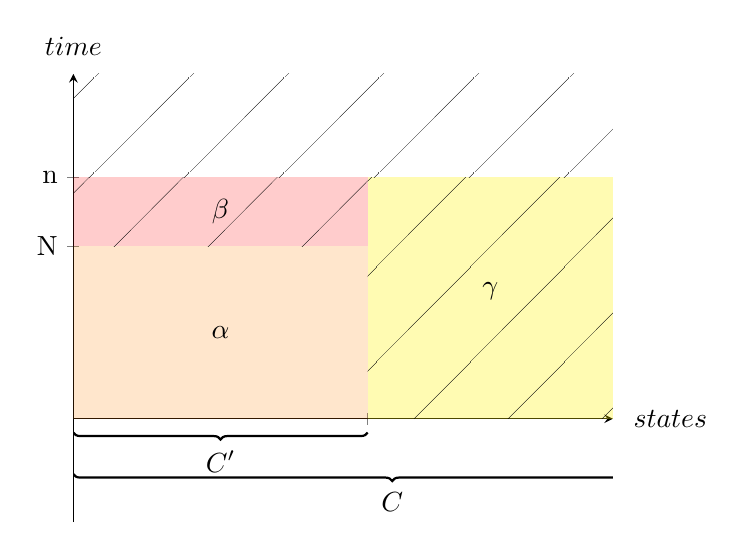
\begin{tikzpicture}
    \newcommand\fign{0.7};
    \newcommand\figN{0.5};
    \newcommand\figCp{0.6};

    \begin{axis}[axis lines=middle,samples=200
            ,ylabel=$time$
            ,xlabel=$states$
            ,xmax=1.1
            ,ymax=1
            ,ymin=-0.3
            ,xmin=0
            ,every axis x label/.style={
              at={(ticklabel* cs:1.02)},
                anchor=west,
              },
            every axis y label/.style={
              at={(ticklabel* cs:1.02)},
                anchor=south,
              },
            ,xtick=data,
            ,xtick={\figCp}
            ,xticklabels={}
            ,ytick=data,
            ,ytick={\figN,\fign}
            ,yticklabels={N,n}
            ]
            \draw [fill=orange,orange,opacity=0.2,draw=none] (0,0) rectangle (\figCp,\figN) node[text=black,pos=.5, text opacity=1]{$\alpha$};
            \draw [fill=red,red,opacity=0.2,draw=none] (0,\figN) rectangle (\figCp,\fign);
            \draw [yellow,opacity=0.3,fill=yellow,draw=none] (\figCp,0) rectangle (2\figCp,\fign);
            \begin{scope}{on foreground layer}    % select the background layer
                \draw[pattern=my lines,draw=none] (\figCp,0) rectangle (2\figCp,\fign) ;
                \draw[pattern=my lines,draw=none] (0,\figN) rectangle (\figCp,\fign) node[black,pos=0.5]{$\beta$};
            \end{scope}
            \draw[pattern=my lines,draw=none] (0,\fign) rectangle (2\figCp,2\fign);
            \node[black,pos=.5,text opacity=1,text width= 2cm] at (axis cs:\figCp,1) {$\gamma$};
            %  underbraces

            \draw[decorate,decoration={brace,mirror},thick]  ([yshift=-5pt]axis cs:0,0) --    node[below=3pt] {$C^\prime$}   ([yshift=-5pt]axis cs:\figCp,0);
            \draw[decorate,decoration={brace,mirror},thick]  ([yshift=-20pt]axis cs:0,0) --    node[below=3pt] {$C$}   ([yshift=-20pt]axis cs:1.3,0);

            \node[] at (axis cs: \figCp+0.25,\figN-0.13) {$\gamma$};
          \end{axis}
  \end{tikzpicture}
% \end{document}
